\documentstyle[epsfig]{book}
% user customisation
% This file defines a few macros for TeX ...  Change them, if you want
% to change the appearence of this document.

% file quote: put a file name in quotes, or print it emphasized, or both:
\newcommand{\fq}[1]{{\em #1\/\em}}

% fragment quote: how do you want fragment names to appear in this document:
\newcommand{\frq}[2]{--\,-- #1: #2 --\,--}

% fragment file quote: specify a Fragment and a file:
\newcommand{\ffq}[3]{--\,-- #1: #2 --\,-- in file \fq{#3}}

% command quote: put a command in a typewriter type font:
\newcommand{\cq}[1]{{\tt #1}}

% command quote quoted: like \cq, but add quotes around the command:
\newcommand{\cqq}[1]{``{\tt #1}''}

% term quote: emphasize an important word or term:
\newcommand{\tq}[1]{{\em #1\/\em}}

% begin/end example quote: use this to indent pieces of code or examples:
\newcommand{\beq}{\begin{quote}}
\newcommand{\eeq}{\end{quote}}


% If you use the cm-fonts, use the following definitions:
%\newcommand{\ttlq}{\`{ }}
%\newcommand{\ttrq}{\'{ }}
%\newcommand{\tthoch}{\^{ }}

% The following defs are ok for the users of Postscript fonts:
\newcommand{\ttlq}{`}
\newcommand{\ttrq}{'}
\newcommand{\tthoch}{\^{ }}

% a list of new commands:
% \backslash prints \
% \leftbrace prints {
% \rightbrace prints }
\begingroup \catcode `|=0 \catcode `[= 1
\catcode`]=2 \catcode `\{=12 \catcode `\}=12
\catcode`\\=12
|gdef|backslash[\]|gdef|leftbrace[{]|gdef|rightbrace[}]
|endgroup

% \leftbracket prints [
% \rightbracket prints ]
% \hoch prints ^
% \underscore prints _
% \dollar prints $
\begingroup \catcode `[= 12 \catcode`]=12 \catcode`^=12
\catcode`_=12
\catcode`$=12
\catcode`"=12
\gdef\leftbracket{[}\gdef\rightbracket{]}\gdef\hoch{^}\gdef\underscore{_}
\gdef\dollar{$}\gdef\dquote{"}
\endgroup

% actually, if a TeX guru sees this file, I would be happy, if he told
% me, how to put these commands into boxes, so that these commands are
% even safe in those cases, that the TeX-Interpreter is called recursively.


\title{b2c - A freeware implementation of the BETA language}
\author{Kai Petzke \\ M\"ullerstr.\ 69 \\ 13349 Berlin \\
        wpp@physik.tu-berlin.de}

\begin{document}
\maketitle

% chapter 0: preface/introduction
\chapter*{Preface}
"What the heck is BETA?"  This is probably the question, that
many people will ask, when they first hear about BETA: "Why do I
want to use BETA instead of going with the mainstream and using
C++?  What makes BETA different?"

I got fascinated, when I first used BETA.  It was around the
time, that I started to look into object oriented
programming.  I had just learned about C++, and I had gotten
disappointed.  The very first thing which I tried to program in
C++ did not work.  If I had a class hierarchie of objects, like
class "lightings", subclass "bulbs", subclass "halogen bulbs", I
wanted to also have a hierarchie of lists of these objects.  That
would mean, that a list of bulbs could be passed to a function,
that needs a list of lightings as argument.  I had to learn, that
this is in principal not possible with C++.  I began to ask
myself: "Why do I want to use a language, which does not even
solve the easiest problem, that I could think of to test it
with?"

Around the same time, I heard about BETA by incident.  And I
found, that one of the examples delivered with the Mjolner
compiler described a BETA solution of my problem.  And shortly
later, I had to learn, that BETA is extremely simple to learn.
To learn C++, you have to read and understand a big book.  To
learn BETA, a short tutorial is enough.

I started to get fascinated.  I don't have to study for long,
and can already use BETA.  And the more I used it, the more
I found out, how versatile it is.  There is only one major
construction element, which is the \tq{pattern}.  Patterns
can do, what functions and classes do in other languages.
And by cleverly combining patterns, patterns can do, what
templates, methods, environments or systems do in other
languages.  There is just this one universal building block,
which does it all for me.  I like this very much.

I hope, that as many people as possible will be able to join
me in having fun with BETA.  Therefore, I have choosen to
write a BETA compiler as freeware, and make it available as
wide as possible.  This document both describes how to use
the compiler, and how the compiler was programmed.

Have fun,
\vspace{3cm}

Kai Petzke


% chapter 1: The BETA language
\chapter{The BETA language}
\section{History of computer languages}
The newcomer, who hears from the BETA language for the first time
may ask just one question: Why BETA?  Why another computer
language?  Aren't C, C++, Fortran, Smalltalk, LISP, Eiffel,
Cobol, BASIC already enough?  Do we really need Babylon?

Apparently, we do.  When comparing human languages to computer
languages, one will find, that computer languages are \em
much\em\/\ inforior than human languages.  This is not
unexpected; human languages have been in use at least 1000 times
as long as computer languages.  However, in one aspect, computer
languages are advanced: they are more precise.  But this is also
a disadvantage --- computer languages do not forgive errors.

Despite the history of computer languages is short, there has
been a rapid development; and fundamental changes happened at
least once a decade.  New features were introduced each time,
and once programmers got used to them, they no longer wanted
to miss them.

The most basic computer languages are assembler languages.  They
consist of a set of simple instructions, like: ``Read the number
stored in memory cell A, and copy it to cell B'', or: ``Read cells
D and F, add their values, and store the result in E''.  Every
single step has to be carried out by hand.  Programming in
assembler is tedious, and the programmer is forced to think of
a lot of things, like which registers carry which values at which
time.  Assembler languages require the programmer to learn a lot
about the machine, which shall be used to solve a given problem.
Assembler languages are in general not portable between different
machines.  When a program is moved to a different architecture,
most, if not all of it, may have to be rewritten.

It was a huge step forward, when the first symbolic computer
languages came out.  They allow programmers to give
human-understandable names to the values used inside a program.
A special program, the \tq{compiler} or \tq{interpreter}, will
translate these numbers into register values.  And because the
compiler can be made to suit different machines, programs written
in symbolic computer languages are portable between different
architectures.  The compiler also takes care of the precedence
of the operators in mathmatical expressions, and will turn
terms like ``$A + 3*(B+C/D) - E$'' into the correct sequence of
assembler instructions.

But programming is still tedious with a symbolic language.  For
example, if a certain expression has to be evaluated at two
points in a given program, it has to be typed twice.  This
problem is fixed by functional or procedural languages like
COBOL or FORTRAN, which allow to isolate expressions and/or
programming statements into functions and procedures, and call
these, whenever needed, instead of writing the same statements
over and over again.  From here, it is only a short step to
introducing libraries, which are collections of often used
subprograms and subroutines.

These two improvements, symbolic and functional languages,
have made it much easier to emit computer instructions, by
using abstract symbolic expressions instead of assembler
instructions, and by allowing the easy re-use of code, that
has been written once.  However, they have not much changed
the way, that data is stored within the system.  A FORTRAN
variable is not much more than an assembler memory cell.  Both
can save a value, and reproduce that value at a later time.
A Fortran array is just a collection of adjanctant memory
cells.

The next steps in advancing computer languages have therefore
been made on the data side, by introducing more abstract data
types than just numbers and characters.  The structures or
records, which languages like C and Pascal provide, allow the
programmer to group values together.  Instead of listing all
the values in the group, for example in a function call, only
a handle for the group (called pointer or reference) has to
be given.

But the possibility to group together values is more than just
a convenience.  In a FORTRAN program, all variables are in
principal the same.  The names, that the programmer choose for
them, may have some meaning to a different human reading the
program, but not to the program itself.  But by grouping
variables together, and by choosing, which variables belong
to a group, the C programmer makes destinctions between the
variables of a program, and this distinction is made available
to the compiling system.  In my opinion, the whole goal of
object oriented computer languages is to make more and more
properties of a variable available to the compiling system.
The hard task is to find those properties, that should be known
to the system, and which don't.  Seen as such, C is already an
(though simple) object oriented language.

This is in contradiction with the most popular definitions of
object oriented languages, which use the presence of inheritence
or subclassing as the key point.  Inheritance allows the
programmer to express, that objects of a new type B are like
objects of an already existing type A, plus a few extensions.
For most people, inheritance is the ``key point'' to object
orientation.  In my point of view, it is just one step in the
task described above: to tell the compiling system as many
properties about a variable as possible.  That a given variable
is derived from another one is sure one of these properties.

Inheritance is easy to realize in many computer languages, because
computer memory is linear, and extending the structure of A
to the structure of B won't affect those memory cells, that
hold the variables for A.  Any function, that has been
written for A will work for B, too.
Quite often, this is not, what people want.  A function, which
does some processing for objects of type A may have to do
some additional or even slightly different processing for
objects of type B.  So virtual functions were introduced,
which perform different operations for different objects.

By making functions dependant on the object type, the
compiling system is given some information about the object.
Again, we are performing our task of giving the compiler more
and more details about objects.

This is by far not the end.  The C++ standard mentions
templates, which allow to group together classes to some kind
of ``super-classes''.  Most operators, like the arithmetic
expressions, may be overloaded for classes as arguments.
Classes may be marked as exceptions, and a few more.

Most of these are rather specific.  The ``+'' operator has few
special meaning to the compiling system.  The programmer of
some class could also choose to overload the ``*'' operator
instead, and that would not change the assembler output
generated by the compiler.  Choosing an operator to overload
or choosing a variable name are quite similiar actions.  They
have a lot of meaning for the programmer, but they do not
affect the compiler itself.

The BETA language follows a different path.  Instead of listing
more and more minute details of a variable or object, it tries
to find the most general properties of the objects in question.

BETA sure has support for grouping values together in structures,
for inheritance and for virtual function calls.  Well, the last
is not really true.  BETA has support for virtual patterns.  A
virtual pattern can be used like a virtual function, but also
like a virtual class.  Yes, BETA allows part or all of the data
which is stored in an object to be virtual, thus depending on the
object type themselves.  This allows an object to be extended in
two dimensions, in contrast to the classical inheritance, which
allows only linear extension at the end.  Virtual objects can be
used as a replacement for C++'s Templates, but that is by far
not their only application.

In C++, all objects ``live'' in the same domain.  Though pointers
between objects may exist, they have no meaning for the C++ run
time system.  It is left to the programmer to keep track of the
relationships between different objects at run time.

In BETA, all objects live inside an environment.  For example,
objects of class or subclass ``ship'' can live inside a ``water''
environment.  That way, any methods defined on the ship object
(like ``move'' or ``load cargo'') can access the properties (like
minimum depth) of the underlying water environment.  The same
is true for cars, which live inside a street environment,
which defines parameters like ``speed limit''.

But what about a car ferry?  BETA allows to stack environments.
Car ferry would be defined as a subclass of ship.  And car
ferry objects would have a part object (or environment), which
is a subclass of street, so that a car ferry can actually load
cars.

In other words: any BETA object can form the environment for
another BETA object.  If object O is in environment E, O can
access all the methods and data defined in E.  If two similiar
objects O1 and O2 reside in different environments E1 and E2,
they may behave differently, depending of the methods of E1 and
E2, which they import.  By making the information about the
environment available to the compiling system, we are back to our
major job of object orientation laid out above.

C++ defines an environment, too, which is the collection of all
globally accessible variables, classes and functions.  But this
rips off any dependency of objects upon the environment.  No
specific environment information can be provided, the compiling
system remains uninformed.


% chapter 2: Overview
\chapter[Overview over the implementation]{Overview
over the implementation of the compiler}
\section{Syntax Definition}
The syntax that this compiler shall understand one day is taken
from the document "The Mjolner BETA System, BETA Compiler,
Reference Manual, August 1994, Appendix B: The BETA Grammar".
Currently, only part of that syntax is implemented, but the
syntactical terms were given the same names as in that document.

\section{Language, Scope}
The BETA compiler is itself written in BETA, with the only
exception being the parser, which was written with a flex/bison
combo and C.  The compiler is not strictly a compiler, rather, it
is a translator, and generates C as output.  I believe, that this
makes development easier in the beginning, as C output is much
easier to check for errors than assembler output.  I hope, that
the compiler will quite soon be able to translate itself into
C, so that it then can be ported to a variety of platforms.

\section{Source tree}
The source of the b2c freeware compiler is shipped in a tar
archive.  When unpacked, it will create a new directory called
\fq{b2c-x.y} or \fq{b2c-x.y.z} in the current directory,
with x.y respective x.y.z being the current version of the
compiler.  At the time of writing this, the current version
is 0.3.

Most file names referenced within this document are relative
to the main BETA source directory.  Inside that directory,
further subdirectories are created:
\begin{description}
\item[\fq{doc}] for storing various documentation.
\item[\fq{runtime}] holds a few C source files and C header files,
    which are needed for compiling and running the C programs
    generated by the b2c translator.
\item[\fq{test}] with example BETA programs.  There are also a
    few scripts, which will compile all the examples with the
    b2c translator, and test, if the compilation went ok, and
    the generated programs work as expected.
\item[\fq{basiclib}] holds basic library files, that are required
    for the compilation of beta programs.
\item[\fq{containers}] holds the container library.  These are
    patterns, that can be used to store lists, stacks, etc. of
    objects.
\item[\fq{src}] is the main source directory of the compiler.
    About one half of the source files are directly located in
    this directory, the other half is located in further
    subdirectories of \fq{src}.
\item[\fq{src/ad}] holds code for parsing Attribute Denotations.
    An Attribute Denotation is the use of a ``variable''.  For
    example, the expression \cq{x+y} contains two
    Attribute Denotations: one is \cq{x}, and one is \cq{y}.
\item[\fq{src/att}] defines functions, whose purpose is to
    handle Attributes.  BETA does not know any difference between
    declaration and definition of a symbol, therefore, the set
    of all possible declarations/definitions have been given
    a new, innocent term: Attributes.
\item[\fq{src/doc}] for documents about the compiler's source
    code, including this manual.
\item[\fq{src/ev}] contains those parts of the compiler, that
    handle the specifics of evaluations.  Evaluations are
    the most general expressions in BETA, which include
    assignments, arithmetic expressions, function calls, etc.
\item[\fq{src/imp}] holds routines for processing imperatives.
    Imperatives are those parts of the programming language,
    that contain the imperative: ``do it''.  So an Imperative
    in BETA is pretty much, what the term ``statement'' has
    been describing for quite some while.
\item[\fq{src/od}] contains auxiliary routines for compiling
    object descriptors.  In the BETA language, an object
    descriptor is the part of a pattern, which describes the
    pattern, which is everything between the \cq{(\#} and the
    \cq{\#)} markers.
\item[\fq{src/virt}] is there for handling virtuals
\end{description}
Please note, that the seperation of the object files into the
subdirectories has not yet been strictly enforced.  For example,
a few files, that process imperatives (like \fq{innerimp.bet}
or \fq{evaluationimp.bet}) are still located in the \fq{src}
directory, not in the appropriate \fq{src/imp} subdirectory.

\section{The main program fragment}
BETA programs can be split into various fragments by use of the
fragment system, and this program, the BETA compiler, uses the
fragment system quite a lot.  The topmost fragment, which must
be present in any BETA program, and which is comparable to the
main() function in a C or C++ program, is called
\frq{program}{ObjectDescriptor}.  In case of this BETA compiler,
it is stored in the file \fq{f2c.bet}.

This file is not long.  An object of type \cq{compiler} is
created.  All arguments, which have been given to b2c on the
command line, are passed to that \cq{compiler} object as
file names, that have to be compiled.

The next step is to traverse the list of file names, that have
to be compiled, and pass each name to the actual compiler.
Because any file may contain the names of further files to
be compiled, this step has to be repeated, until no files are
left.  It would be wrong to assume, that only the files given
on the command line shall be compiled.

The last step is to link all the object files generated during
compilation into an executable.

\section{The main pattern of the compiler: compiler}
The main pattern of the compiler, called \cq{compiler}, is found in
the file \fq{compiler.bet}.  It holds a few important attributes,
which represent the current state of the compiler:
\begin{description}
\item[fl] (\underline{f}ile \underline{l}ist) A list of files, that
        has already been compiled.
\item[ol] (\underline{o}bject \underline{l}ist) The list of object
        files, that will have to be linked in the last step.
\item[tl] (\underline{t}odo \underline{l}ist) The list of files,
        that needs to be compiled, but has not yet been processed.
\item[fc] No BETA file may be read twice, even, if it is accessed
	with two different filenames.  The FilenameConverter system,
	which is instantiated in the \cq{fc} item, keeps
	track of all files, that it has seen so far, and ensures,
	that it gives back the same pathname each time a given
	file is accessed.
\item[sl] (\underline{s}lot \underline{l}ist) A list of all slots
	in all input files.
\item[nameTable] A hashTable, which holds information about all the
	names declared in the various Attributes of the currently
	compiled BETA program.
\item[errstream] An output stream to that error messages can be
	printed.
\item[mainorigin] This is a reference to the file, which holds the
	\frq{BETAENV}{ObjectDescriptor} pattern, that is the
	common environment to all BETA programs.  Any BETA
	program instantiates one, and only one, object from this
	pattern.
\item[mainobject] A pointer to the object descriptor in the
	BETAENV fragment, which defines the \cq{Object} pattern.
\item[c\underline{\ }file] A pointer to the currently processed BETA source file.
\item[slotlist] A pointer to a list of all slots, that have been
	encountered by the compiler so far.
\item[cintf] This Attribute holds parameters about how the C output
	should look like.  It depends mostly on the C compiler, that
	you use.  See file cintf.bet for details.
\item[opt] Compiler options, see file \fq{option.bet}.
\item[od3] Pointer to an object descriptor.  This is used during
	phase 3 of the binding/checking algorithm (see
	section \ref{check-phase3}) for referencing the
	currently processed object descriptor.
\item[odserial] This counter is increased every time, that an
	object descriptor is found during parsing of a file.
\end{description}


\section{The Parser}
Actual compilation is performed by the routines in
\fq{compile.bet}.  They take a filename and a starting directory
as argument.  These two are combined into a standardized pathname
via the FilenameConverter.  If that file has not already been
processed, a new BETAfile object is generated for that filename,
and the parser is invoked.  The parser itself is divided in two
halfes: the FragmentLanguageParser (in \fq{fragparser.bet} and
\fq{fragparserbody.bet}) reads the fragment language headers of a
file and directly interprets them.  For example, an INCLUDE
directive results in a recursive call to the compiler, so that
the included file is read in and compiled before the main part of
the current file.

After the fragment headers have been processes, the main parser
(in \fq{parser.bet}, \fq{parserbody.bet}, \fq{parse.y} and
\fq{read.l}) may be invoked to read the rest of the file.  This
invocation is omitted, if b2c can find a more recent \fq{.o}
file, that corresponds to the current \fq{.bet}.  However, if
the current file is included by another source file, and that
other source file has to be recompiled, parsing the current
file cannot be left out.

The parser is rather simple, as it performs only syntax checking.
All grammatical checks are left for later.

\section{Binding and Checking Phases}
\label{check}
\label{check-phase3}
After a file has been parsed, the next step is to bind and
check the contents of that file.  Binding means to find free
slots for all the fragments, that were contained in a source
file.

Checking means to find and report all grammatical errors by
traversing the source code tree.  During the late phases of
checking, all BETA expressions, evaluations and imperatives are
reduced into an ordered list of C statements and expressions.

Due to the nature of the BETA language, the grammatical checking
is not a straightforward process like in C, which can be
performed token by token while the parser reads a source file.
Rather, checking is performed in a number of distinct phases.
Each phase traverses the source code tree in a different order.
During the reduce phase, it may happen, that some nodes of the
source code tree are hit more than once:

\begin{description}
\item[resolve] The first phase is to resolve all name references
    like attribute denotations or remotes.  This requires two
    actions:
    \begin{itemize}
    \item Whenever a pattern is first hit during the traversal
	of the syntax tree, all the names defined in its
	attribute section are entered into a global name
	table.  While this is done, those names, that have
	been declared twice, are detected and reported.
    \item Try to find the corresponding declaration for all
	attribute denotations and remotes.  Report all
	references to undeclared names.
    \end{itemize}
    While resolving name references, it is often required to
    jump forth and back in the source code tree:
    \begin{itemize}
    \item In case of a remote like \cq{P.Q}, we cannot resolve
	\cq{Q}, before we actually know, what type of object
	\cq{P} is.  That does not only require to resolve \cq{P},
	it also requires to resolve any denotation, that is
	contained in the declaration of \cq{P}:
	\begin{quote}\begin{verbatim}X: ^P.Q;
P: @pattern;
pattern: (# Q: (# x,y: @integer #) #);
\end{verbatim}\end{quote}
	In this example, resolving the topmost denotation
	\cq{P.Q} requires to process \cq{P} first.  Because
	\cq{P} is itself defined as a reference, that reference
	has to be resolved, too, or the part \cq{.Q} in the
	expression \cq{P.Q} would not be understood.  So, in
	order to check the declaration of \cq{X}, we are forced
	to also process the declarations of both \cq{P} and
	\cq{pattern}, which appear later in the source file.
	This is different to traditional computer languages like
	C++, Pascal or Fortran, where the syntactical checking is
	a straightforward process.  In case, that an object is
	used before it is defined, these languages require a
	forward declaration, which is neither possible nor
	necessary in BETA.

	For the most part, that feature is just convenient to the
	BETA user.  But there is also a new class of syntactical
	error introduced.  It shows up in incomplete
	declarations, where objects depend upon each other.  This
	will lead to an illegal recursion in the compiler's
	resolving function:
	\begin{quote}\begin{verbatim}A: ^B.obj;
B: ^A.obj;
\end{verbatim}\end{quote}
	Resolving \cq{A} requires to first process \cq{B}.
	Resolving \cq{B} requires to first process \cq{A}.  As a
	result, neither can be completed.  To detect such illegal
	recursions, each attribute denotation holds a tri-state
	flag, which tells, if resolving that attribute has not
	yet been done, is in progress, or has been completed.
    \item When a declaration for a name is not found in the
	pattern, that it was used in, it is next searched for in
	the superpattern of that pattern.  So that superpattern
	has to be found before we continue looking for that name.
	In case of normal patterns, the superpattern is defined
	by a prefix, which itself is an attribute denotation.
	This leads to another case, where resolving a denotation
	requires to first resolve another denotation.

	In case of virtual patterns another level of complexity
	may be added.  Finding the superpattern for a virtual
	binding declaration requires to search through the
	superpatterns of the pattern, that holds the virtual
	binding declaration.
    \end{itemize}

%\item[super] Find the super pattern for each pattern.  This is
%    a bit tricky, as looking up a superpattern changes the
%    name space, and thus affects the process of looking up the
%    superpattern.  See the following example:
%    \begin{quote}\verb+A: IntegerValue (# do 1->value #);\\
%	\verb+B: C (# V: A (# do value+1->value #) exit V #);+\\
%	\verb+C: (# A: IntegerValue (# do 2->value #) #);+
%    \end{quote}
%    It must be made sure, that B.V is derived from the method
%    C.A, not from the pattern A.  This is true, if the
%    superpattern of B is looked up before that of B.V.
%
%    If dynamic references are allowed in the Prefix part of an
%    object descriptor, the grammar may get ambigious:
%    \begin{quote}\verb+P: @A+\\
%	\verb+A: P.M (# M: X (# #) #);+
%	\verb+X: (# X: (# exit 2 #) exit 1 #);
%    \end{quote}
%    The question is: which pattern does the \cq{X} in \cqq{M: X
%    (\# \#)} refer to?  There are two solutions, and both lead
%    to a contradiction:
%    \begin{itemize}
%    \item The \cq{X} in \cqq{M: X} could refer to the pattern,
%	which is declared as \cq{X}.  But then, \cq{P.M} is a
%	subpattern of \cq{X}, so all references to \cq{X} in that
%	pattern, namely the \cqq{M: X}, should refer to \cq{X.X},
%	not \cq{X}.
%    \item The \cq{X} in \cqq{M: X} could refer to the method
%	\cq{X.X}.  But then, \cq{P.M} is a subpattern of
%	\cq{X.X}, and \cq{X} is undefined inside \cq{P.M}.
%	So the \cq{X} in \cqq{M: X} must refer to the global
%	pattern \cq{X}, not \cq{X.X}.
%    \end{itemize}
\item[follow] The next step during checking is to follow all
    static references and inserted items as well as
    superpatterns.  This is required to detect illegal recursions
    like the following:
    \begin{quote}\begin{verbatim}P: (# A: @P #);
\end{verbatim}\end{quote}
    In this case, the pattern \cq{P} contains a copy of itself.
    In particular, all the following static links are followed
    during the follow check:
    \begin{itemize}
    \item A static reference declarations like:
	\begin{quote}\tt\tq{name}: @\tq{pattern};\end{quote}
	creates a static link from the pattern, in whose
	attribute section it appears, to the \tq{pattern}
	used in the declaration.
    \item Inserted items in the do, enter or exit part of a
	pattern create static links from that pattern to the
	inserted item.
    \item The prefix of a pattern declaration:
	\begin{quote}\tt \tq{pattern}: \tq{prefix} (\# \ldots\ \#)
	\end{quote}
	statically links \tq{pattern} to \tq{prefix}.
    \end{itemize}
    Many of the properties of a pattern, like the list of
    pointers to enclosing objects, or the list of virtuals,
    depend on the superpattern of that pattern.  All these
    properties are set during the follow phase. Performing a
    follow check on a pattern requires to perform a follow check
    on the superpattern --- and after that has been completed, we
    can be sure, that the properties of the superpattern are up
    to date and may be copied to the pattern.

    Finally, the follow phase is used to create a set of ordered
    lists of all objects, functions, patterns, etc.\ in a BETA
    source tree.  These lists are used later to create correct
    C source code, where no object may be used before it has
    been declared respective defined.
\item[complete] This phase completes the check of the follow
    phase.  It traverses the source code tree in the syntactical
    order, and starts a follow phase check on all object
    descriptors, which have not been subject to that check, yet.
\item[reduce] All BETA expressions are reduced to "flat" C
    expressions during this phase. For example, an assignment
    \cq{A -> B} is split into several sub-actions, depending
    on the type of \cq{A} and \cq{B}:
    \begin{itemize}
    \item Create an object of type A.
    \item Call the do part of A.
    \item Create an object of type B.
    \item Assign all elements on the exit list of A to the
	    according enter list elements of B.
    \item Call the do part of B.
    \end{itemize}
    Further complication may result, if the exit part of A
    and/or enter part of B contain more references to
    non-simple objects or patterns.  In that case,
    reduction has to be performed recursively, and may
    result in an illegal recursion, if enter or exit lists
    of different objects contain references to each other.

    The reduce phase is also responsible for enforcing type
    safety in all assignments and reference computations.
    Qualification errors are reported, and run time qualification
    checks are inserted where appropriate.

    The reduce phase should also insert implicit checks for
    pointers to be non-null, whereever appropriate, so that
    compiled BETA programs will detect dereferencing a NONE
    reference at run time.

    The reduce phase is the first phase, which does not traverse
    the whole source tree.  Rather, a list of the expressions,
    that shall be reduced, is generated during one of the earlier
    checking phases.
\item[extra] Some special expressions (currently only calls to
    external functions) need one more level of checking after
    reduction has been completed.  Again, this check is performed
    only for those objects, that have been entered into a special
    todo list.
\end{description}

If two phases of the checking process do not interfere with each
other, they can be performed during the same traversal of the
source code tree.  In the current implementation, the complete
phase will also perform all resolve and follow checks.  You can
think of the complete phase of being a machine, that traverses
the source code tree, thereby triggering all necessary follow
and/or resolve checks.

Further versions of the compiler will do a number of optimization
phases after checking has been completed.

\section{Code generation}
If the checking phase found no errors, the next step is to actually
generate C output.  Special care has to be taken to emit the
various declarations in the correct order, so that all C
structures and functions are declared, before they are actually
used in another declaration.
That is achieved by using the follow phase of checking to create
ordered lists of the actions to be performed during code
generation.

Code is emitted into two files.  A \fq{.h} file holds the
declarations of the structures and functions for a given BETA
source file.  The beginning of a \fq{.h} file also holds the
\cq{\#include} directives, if necessary, for other generated
\fq{.h} files.

The actual definitions of the structures and functions are
written to a \fq{.c} file, which \cq{\#include}'s its own \fq{.h}
file.  After both files have been written, a C compiler is
invoked to compile the C source code into an object file.

If for a given \fq{.bet} source file, a \fq{.c} and \fq{.h} file
can be found, and have a modification date, which is newer than
that of the \fq{.bet} file, code generation is omitted.  If also
a \fq{.o} file is found, which is newer than the \fq{.c} and
\fq{.h} file, calling the C compiler is omitted, too.


% chapter 3: Patterns, Objects and DO-Parts
\chapter{Patterns, Objects and DO-Parts}
\section{Pattern structure}
All standard BETA objects have to carry around a certain amount
of run time type information.  Rather then including this
information into each object, most of it is collected into a
static structure at compile time.  The objects themselves
therefore only need to carry a pointer to that structure.  This
pointer is located at a fixed position at the beginning of
an object's structure; currently this pointer is the first
element of an object.

\subsection{Pattern relationships}
BETA defines certain relationships between patterns, respective
the objects generated from them.  Any given pattern $P$ has a
superpattern $S(P)$.  The single exception is the \cq{Object}
pattern, which has no superpattern.  However, \cq{Object} is the
implicit superpattern of all patterns, whose supperpatterns were
not specified.

Every pattern $P$ also has a statically enclosing pattern $E(P)$.
$E(P)$ is the pattern, whose attribute section holds the
declaration of $P$.  There are two exceptions: the enclosing
pattern of \cq{Object} may be any pattern or empty.  And because
\cq{Betaenv} always is the outermost pattern, its enclosing
pattern is not defined, either.

One might assume, that a pattern $P$, and its superpattern $S(P)$
have the same enclosing patterns, so that $E(P)$ = $E(S(P))$.  But
this is in general not true in BETA.  A common example are virtual
patterns:
\begin{quote}\begin{verbatim}env: (# virt1:< (# ... #) #);
myenv: (# virt1::< (# ... #) #);
\end{verbatim}\end{quote}
Clearly, the \cq{virt1} pattern of \cq{env} has \cq{env} as
enclosing pattern, while the \cq{virt1} pattern of \cq{myenv}
has \cq{myenv} as enclosing pattern.  However, in this special
example, the equation: $E(S(\cq{myenv.virt1})) =
S(E(\cq{myenv.virt1}))$ holds true.  These and some other
relationships will be detected by the compiler, and used for
various optimizations.  But the general situation in BETA
is, that any pattern $P$ has
a set of enclosing patterns $E(P)$, $E(S(P))$, $E(S(S(P)))$,
\ldots, $E(S^n(P))$, where $S^n(P)$ is the n-th superpattern
of $P$.

\subsection{Definition of \cq{struct pattern}}
All required run time type information is stored in a special
pattern structure.  Objects only hold a pointer to that structure
instead of reproducing the run time type information over and
over again.

Like object size may vary, the size of the run time type
information is not fixed either, but depends on the details of
the pattern, like the number of virtual methods used.  However,
the first few fields of the structure are well defined for (almost) all
patterns.  This common header is defined as \cq{struct pattern}
in the header file \fq{beta.h}:
\beq\begin{verbatim}/* standard structure for storing patterns */
struct pattern {
    const struct pattern *super;
    const struct pattern *outer;
    int len;
    int outerindx;
    int (*function)(void *const th);
    void *(*newf)(void *const th);
};
\end{verbatim}\eeq

The meanings of the fields are as follows:
\begin{itemize}
\item \cq{super} is a pointer to the superpattern of this pattern,
    introduced as $S(P)$ in the notation above.
\item \cq{outer} refers to the structure of the enclosing pattern $E(P)$.
\item \cq{len} is the length of the objects, that can be generated
    from this pattern, in bytes.
\item \cq{outerindx} is an index into the objects generated from
    this pattern.  It denotes the location, where the pointer to
    the enclosing object $e(o)$ of that object is stored.
\item \cq{function} is the first slot of the call table for the
    various DO parts of this patterns and its superpatterns.  In
    the case of empty or only trivial DO parts, the value zero
    will be stored here; otherwise this cell will contain the
    pointer to a function, which executes the complete DO part
    of this pattern and its superpatterns.  This function requires
    one argument, which must be a pointer to an object generated
    from this pattern.

    After successfull completion of the directives in a DO part,
    this function will return the value zero.  If an leave or
    restart imperative occurred, which could not be catched in
    the DO part itself, a handle for that imperative will be
    returned.  It is the responsibility of the caller to test
    the return value and to process the leave/restart handles.
\item \cq{newf} is a pointer to the object generator function.
    As even the most trivial objects have an object generator
    function, this pointer is never zero.  Object creator
    functions take exactly one argument, which is a pointer
    to the enclosing object of the newly created object.
    This argument must be nonzero, except, if the creator of
    the \cq{Betaenv} object is called.  In either case, this
    function will return a pointer to the newly generated
    object.
\end{itemize}

\section{Objects}
Storage of BETA objects is different from that of the patterns.
While a pattern and its superpattern are stored in different
structures, an object and its ``superobjects'' are always unified
into one structure.  The first element of an object is always a
pointer to the pattern structure for that object, then follow the
data fields and pointers, that were declared in the attributes
sections of the relevant pattern and its superpattern(s).  The
fields declared in the outermost superpattern come first, then
those declared in the second outermost superpattern, and so on.
So declaring a subpattern of a pattern will extend the object
structure at the end, while the rest of it is unchanged.

To keep track of the size of an object, the pattern structure
holds the field \cq{len}, which stores the length of the
complete object structure of an object generated from that
pattern.

\subsection{Relations between enclosing objects, and reuse of pointers
    to them}
While an object and its ``superobjects'' are always inlined into
one structure, an object and its enclosing objects are not.
Rather, any object holds a set of pointers $e_1$, \ldots\ $e_n$
that point to the enclosing objects.  The compiler tries to
minimize the number of these pointers to enclosing objects
by re-using them in a few cases, like when two enclosing
objects are the same: $e_k = e_i$, or superpatterns of each
other: $e_k = s^j(e_i)$.  In both cases, $e_k$ can be omitted.

Inside the C structure of the object, these pointers are
named \cq{encl1}, \cq{encl2} and so on.

In general, for any item in the superpattern list of a pattern, a
different pointer to an enclosing object is needed.  However,
these pointers often denote the same object, and it is wise to
apply a few rules to reduce the number of pointers needed:
\begin{itemize}
\item Even though the enclosing pattern of the \cq{Object}
    pattern is undefined, objects of type \cq{Object} still need
    a pointer $e_1$ to an enclosing object.  Otherwise, the
    system would not be able to perform qualification checks at
    run time.

    But because the \cq{Object} pattern does not define any
    meaning to the enclosing pointer $e_1$, any direct subclass
    of \cq{Object} can recycle that pointer $e_1$ for their
    own purposes, instead of defining a new $e_2$.

\item If a pattern and a subpattern are defined inside the same
    attribute section, they have the same enclosing pattern.
    Objects generated from these also have the same enclosing
    object, so the enclosing object pointer can be reused.

\item Another common situation is, that the enclosing pattern of
    the superpattern of $P$ is a superpattern of the enclosing
    pattern of P: $E(S(P)) = S^n(E(P))$, with $n \ge 1$.
    This is typically the case with virtuals:
    \beq\begin{verbatim}P: (# V:< (# ... #) ... #);
Q: P (# ... #);
R: Q (# V::< (# ... #) ... #);
\end{verbatim}\eeq
\end{itemize}
After these rules have been applied typically only one or two
pointers are left.  But even these are not independant.  If you
have the enclosing object $e(o)$ of an object $o$, the enclosing
objects of the superpattern parts of $o$ (like $e(s(o))$,
$e(s(s(o)))$ and so on) can be determined by using a
recursive scheme:
\begin{itemize}
\item If $o$ is of type \cq{Object}, we are done, as \cq{Object}
    has no superpattern, thus no $e(s(o))$ can be determined.
\item If $o$ is generated from a pattern, that is a direct
    subpattern of \cq{Object}, $s(o)$ is of type \cq{Object}.  So
    any object may serve as $e(s(o))$, and we set $e(s(o)) =
    e(o)$, by applying the first pointer reuse rule above.
\item In any other case, $o$ must have been generated from a
    pattern $P$, that has an explicit superpattern $S(P)$.
    $S(P)$ is denoted using a \tq{prefix} in BETA:
    \beq\tt P: \tq{Prefix} (\# ... \#)
    \eeq
    The \tq{Prefix} can be defined in one of three ways:
    \begin{enumerate}
    \item If \tq{Prefix} is a simple pattern name, it must be
	defined in any of the enclosing patterns of $P(o)$, like
	$E(P(o))$, $E(E(P(o)))$, and so on.  Otherwise, that
	pattern name would be an illegal name reference.  So
	$E(\mbox{\tq{Prefix}}(P(o))) = E(S(P(o)))$ must be equal
	to $E^n(P(o))$, with $n \ge 1$.  To get the corresponding
	enclosing object, simply leave out the pattern lookup:
	$e(s(o)) = e^n(o)$.
    \item If \tq{Prefix} is of the form
	\tq{attribute-denotation}.\tq{pattern-name}, things are
	even easier.  \tq{attribute-denotation} must denote an
	object, and this object is the enclosing object of the
	prefix, thus that of the superpattern.
    \item In case of a virtual binding, the prefix is given as
        the preceding virtual declaration or virtual binding,
	which must be present in a superpattern of the enclosing
	pattern.  So: $e(s(o)) = s^n(e(o))$ for some $n \ge 1$.
    \end{enumerate}
\item Repeat the above scheme with $s(o)$ instead of $o$ to
    determine the enclosing object $e(s(s(o)))$.
\end{itemize}
Summarization: only $e(o)$ is required to generate the full set
of pointers to enclosing objects $e(s^n(o))$, with $n \ge 0$.
Thus the term "the enclosing object" will be used from now on to
refer to $e(o)$.

\subsection{Full type qualification}
From what was said before, we can conclude, that two pieces of
information are required to fully qualify the type of an object
in BETA:
\begin{itemize}
\item A pointer to the pattern $P(o)$.
\item A pointer to the enclosing object $e(o)$.
\end{itemize}

\subsection{Static and dynamic references}
BETA objects may contain static and dynamic references.  There are
two possible methods of implementation:
\begin{itemize}
\item Store a pointer to the object denoted by this reference in
    the object structure.
\item Inline the denoted object into the object structure.
\end{itemize}
Inlining in general is the more performant choice.  However,
inlining is not possible in quite a few cases:
\begin{itemize}
\item Dynamic references can never be inlined, because the denoted
    object may be changed by a reference assignment.
\item Static references to virtual patterns cannot be inlined,
    because in a subclass, the virtual might be extended, and
    would then no longer fit into the place, that has been
    reserved for it in the inlining process.
\item Static references to object descriptor slots cannot be
    inlined, either.
\end{itemize}
If none of these rules apply, inlining is performed.

\subsection{Generating objects}
When a BETA object is generated, the following actions have to be
performed:
\begin{itemize}
\item Allocate sufficient memory.
\item Clear that memory, so that all numbers are initialized to
    zero, all booleans are set to false and all references point
    to NONE.
\item Set the pointer to the pattern structure.
\item Set the pointer(s) to the enclosing object(s).
\item Initialize all static references of this object.
\end{itemize}
Especially the last two actions (setting the pointers to the
enclosing objects and initialising all static references) are
rather object specific.  It is hard to operate them from a table.
Therefore, the compiler emits a specific object generator
function for each pattern.

This function takes just one argument, which is the pointer to
the enclosing object.  All other information, like the pointer to
the pattern structure, the lookup of the complete list of
enclosing objects and the initialization of the static references
are hardcoded into the function.

In the last step, when static references are initialised, an
object generator function may (and sometimes has to, especially,
when virtuals are involved) call other object generator
functions.  However, when  object generator functions call other
object generator functions, they will never loop, as recursive
static references, where an object contains itself, are forbidden
in BETA for obvious reasons.

The exception to this rule is caused by repetitions: the
definition of a repetition contains a general BETA expression,
which calculates the initial size of the repetition, and this
expression may well cause recursive calls of the object creator
function.

Generating objects in general has very few side effects.  In most
cases, despite the allocation of memory, no other global data is
changed.  The exception are cases, where the \tq{prefix} of a
pattern or a static reference is a computed remote, a reference
lookup or similiar.

\subsection{Generating objects from virtual patterns}
BETA's virtual pattern can be used in two different ways:
\begin{itemize}
\item Their type can be queried, either explicitely with the
    operator \cq{\#\#} or implicitely in a run time qualification
    check.  In this case, the virtual pattern is used as a virtual
    type.
\item They can be used to instantiate BETA objects with the
    operator \cq{\&}, in a declaration or in an inserted item.
    After object generation has been completed, the DO part may
    be called.  This means to use the virtual pattern like a
    virtual function.
\end{itemize}
These operations are not independant of each other.  If we have
queried the full type of a virtual, we can always use the type
information to directly generate an object from it.  And if an
object has been created, the type can be queried from it, too.
However, object generation may have side effects, so it is not a
good idea to perform it, unless it is required explicitely.

The full type qualification of a virtual $v$ consists of the
pattern $P(v)$ and the enclosing object $e(v)$.  While the
pattern information could be retrieved by a simple indirect table
lookup into the environment of the virtual, the enclosing object
$e(v)$ can be a somewhat arbitrary function of that environment.
Therefore, we need a C function to do the virtual type lookup.
It takes two parameters on input: a pointer to the object, in
which the the virtual is to be looked up, and a pointer to
storage space for the full type qualification.  As a convenience
and for efficiency, if the later pointer is NULL, an object with
the type of the virtual will be generated and a pointer to the
object is returned.

\subsection{Destroying objects}
There is no method or function in BETA, which can be used for
destroying an object.  Rather, the compiler and runtime libraries
are responsible for keeping track which objects are still in use.

In special cases, the compiler might already be able to determine
at compile time, that a given object has a limited lifetime, and
allocate it in a space, where it can be easily deallocated, like
on the stack.  In general, though, the compiler cannot know, how
long an object will be around.  It is therefore necessary at run
time to examine, which objects are no longer used, and reclaim
the storage allocated to them.  This process is called
\tq{garbage collection}.

An experimental version of a garbage collector has been
implemented by Jan Okrouhly.

\section{Calling an object's DO-part}
\label{call-do-part}
In procedural languages like C, calling a function means, that
this function will first allocate some local storage on the stack,
then execute some code, deallocate the storage, and return.  This
is not true for BETA.  Generating the storage for an object, and
calling a DO--Part are very well distinct processes.

In procedural languages, passing parameters between a calling and
a called function is a shared process: the calling function will
store the values of the parameters in a reserved region (like
processor registers or the stack), and the called function will
pick them up there - and later put the return value in the same
or another reserved region.  This is not true for BETA.  For
example, the caller may only provide an incomplete set of
parameters to the called function, as in the following example:
\begin{quote}\begin{verbatim}env: (#
   f1: (# A: @integer enter A do A->putint; INNER #);
   f2: f1
     (# B: @integer
     enter B
     do ' '->put; B->putint; INNER
     #);
   X: ^f1
do
   &f2[]->X[];
   1->X
#);
\end{verbatim}\end{quote}
Here, the call \cq{1->X} will execute the joint do part of
\cq{f1} and \cq{f2}, but processes only the ENTER part of
\cq{f1}.  Therefore, the ENTER and EXIT directives are completely
processed in the calling function, not in the called function.
The general calling sequence for the Do-Part of a pattern
therefore reads as follows:
\begin{enumerate}
\item Generate the object, that shall be called.
\item Process the ENTER part.
\item Call the code, that processes the imperatives of the do part.
\item Process the EXIT part.
\end{enumerate}
Any of these steps is optional, depending on the exact form of the
expressions in the call.

\subsection{Executing the INNER imperative}
The INNER imperative is a placeholder, where the imperatives of a
subpattern will later be inserted.  There are two options on how
to translate the nested do parts of a pattern and its superpattern
to C functions:
\begin{itemize}
\item The compiler recursively interprets all INNER imperatives,
    and generates code, which executes the complete do part of a
    pattern --- from the outermost superpattern to the pattern
    itself.  However, this scheme may result in large executable
    programs, as the object code of the do-part of a given
    pattern has to be repeated in all subpatterns of that
    pattern.

    To execute the do part of a given object, the specific
    function for that object's type has to be called.
\item The compiler replaces all INNER imperatives with an
    indirect function call of the appropriate INNER function.  No
    code repetition is necessary in this case, but the indirect
    function call causes delay, and the indirect function call
    table increases the size of the pattern structure.

    To execute a DO part, the DO part function of the
    outermost super--object has to be called; this function
    will automatically call all INNER functions via the
    indirect call tables.
\end{itemize}

Currently, the indirect call scheme has been implemented.  In a
later version of the compiler, it should also support the
inlining of INNER parts.  Depending on some heuristics, like the
size of the resulting function, the compiler should decide,
which scheme to use.

\subsection{Handling of empty and trivial DO parts}
Many BETA objects have an empty DO part.  No function call is
generated by the compiler for them.

Other BETA objects, namely abstract superpatterns, have trivial
DO parts, that contain nothing but one INNER imperative.  The
most prominent such pattern is the \cq{Object} pattern.  For
these patterns, no function is generated, either.  The call table
slot is left open, until a subpattern defines a non-trivial DO
part.

In some cases, where the DO part of a dynamic reference is to be
executed, the compiler may not know at compile time, which
function to call or whether to call a function at all.  In that
case, an indirection through the first slot of the call table is
performed, which is very similiar to the lookup of INNER.

\subsection{LEAVE and RESTART}
There are two more BETA imperatives, that affect the flow of
execution in non-standard ways: LEAVE and RESTART.  In many
cases, they can be handled locally and translated into a goto
statement in C, like where a loop is restarted or left.

However, LEAVE and RESTART can also be used to return control
to a specific function on the call stack.  In these cases, two
informations have to be provided:
\begin{itemize}
\item A pointer to the object, whose DO part should catch the
    LEAVE or RESTART.  That object's DO part must be on the
    calling stack --- or a run time error will occur.
\item A unique identifier, which denotes the label inside the DO
    part, which shall be restarted or left.
\end{itemize}
These two informations are combined into a leave/restart handle.
The identifiers are implemented as pointers to predefined
character strings.  That way, we easily ensure that no identifier
value is repeated.  Also, the character string can hold details
about the actual operation being performed, which make the error
message more verbose in case, that the complete stuck is unwound
in a LEAVE or RESTART.

The current BETA syntax is quite strict, in that a leave or
restart statement may only occur in the DO part of a given
pattern.  Therefore, the following is illegal:
\begin{quote}\begin{verbatim}interpreter:
  (#
     abort: (# do leave interpreter #);
     syntax_error:
       (# do 'Syntax error!'->putline; abort #);
     read_token:
       (#
       do
          ...
          (if some_error_condition then syntax_error if)
          ...
       #);
  do
     read_token;
  #)
\end{verbatim}\end{quote}
However, the following will work:
\begin{quote}\begin{verbatim}interpreter:
  (#
     abort: (# do throw_it #);
     throw_it: ^Object;
     syntax_error:
       (# do 'Syntax error!'->putline; abort #);
     read_token:
       (#
       do
          ...
          (if some_error_condition then syntax_error if)
          ...
       #);
  do
     l1:
       (#
       do
          &(# do leave l1 #)[]->throw_it[];
          read_token;
       #);
  #)
\end{verbatim}\end{quote}
The advantage of the strict syntax is, that we will know at
compile time, which LEAVE/RESTART imperatives may occur, and
which will not.  So we can restrict the number of handles to the
required minimum.  In the first example, the \cq{abort} method
might be defined in a different fragment in a different source
file, and the run time system might be quite surprised to receive
a handle for the \cq{leave interpreter} imperative.

\section{Special Object Descriptors}
As any other language, BETA needs a set of basic types and basic
functions respective methods on which it can operate.  An example
of a basic type is \cq{Integer}, a basic method is the
\cq{extend} method of a repetition.  A common feature of these
basic types and functions is, that they cannot be represented
within the language itself.

Most languages therefore define a set of keywords for these types
and functions, like the type \cq{int} or the function
\cq{sizeof()} in C.  This is not true in BETA.  There are no
keywords reserved for the basic types.  It is therefor possible
to redefine names like \cq{Integer} in your own patterns.

However, the compiler must still be able to recognise the basic
types.  Therefore, certain pattern names are given special
meaning --- but only in the outermost fragment, that is typically
called \cq{betaenv}.  The list of special names is:
\begin{quote}
	Boolean \\
	Char \\
	Integer \\
	Real \\
	Shortint \\[2ex]
	Data \\
	External \\
	Object \\
	Repetition \\
	Text
\end{quote}

Most special descriptors are accounted for in the fragment
\ffq{PatternDeclCheck0}{DoPart}{attributebody.bet}.  The single
exception is the \cq{Object} pattern.  Because it is the
superpattern of all other patterns, it has to be checked before
any other pattern is processed.  This special treatment of the
name \cq{Object} is performed in
\frq{PatternDeclCheckName}{DoPart}.

\subsection{The basic types}
The five patterns \cq{Boolean}, \cq{Char}, \cq{Integer},
\cq{Real} and \cq{Shortint} all represent a storage cell, which
holds a value.  To generate an object from one of those patterns
means to allocate an appropriate storage cell.  To enter an value
into that object means to put that value into the storage cell.
To exit a value from the object means to retrieve the value
stored in that cell.  In neither case, a DO-part is executed.

To ensure type safety without sacrificing efficiency, all
references to objects of these basic types must be static
references.  That means, that these objects are well defined
within the enclosing pattern, and only within that pattern.
Objects of the basic types don't have a pointer to the pattern
information or to the enclosing object.

The backdraw is, that the basic types cannot be extended in any
way.  No subclassing, no further attributes, no DO-Part is
possible.  To partly overcome that shortage, the basic library
\fq{betaenv.bet} defines full pattern versions
\cq{IntegerObject}, \cq{CharObject}, \ldots\ of the basic types.

\subsection{The \cq{Data} pattern}

\subsection{The \cq{External} interface}

\subsection{The \cq{Text} type}

\subsection{The main superpattern: \cq{Object}}

\section{Repetitions}
The repetitions defined by BETA are more than just plain arrays.
Rather, many of the operations on repetitions resemble the
behaviour of specialized patterns respective objects:
\begin{itemize}
\item Certain methods (namely \cq{new}, \cq{extend} and
    \cq{range}) operate on repetitions pretty much like "normal"
    methods on conventional objects.
\item Repetitions have an exit list, that will exit the values of
    all the elements in the repetition.
\item Repetitions have an enter list, that can accept the elements
    exited from another repetition.
\item The size specifier in a repetition declaration may be any
    valid BETA expression.  Evaluating that expression may have
    side effects on other BETA objects.  Normal object generation
    does not have such side effects.

    In other words: the size specifier adds functional aspects
    to a repetition, like the do part adds functional aspects
    to a pattern.
\end{itemize}

This compiler actually implements BETA repetitions by turning them
into patterns.  Directly after scanning the declaration of a
repetition:
\begin{quote}\tt \tq{name}: [\tq{expression}] @\tq{type}
\end{quote}
it is turned into the following:
\begin{quote}\verb+repetition:+\\
   \verb+  (#+\\
   \verb+     size: @integer;+\\
   \verb+     elsize: @integer;+\\
   \verb+     range: (# exit size #);+\\
   \verb+     new: (# enter size do (* +{\it create repetition}\verb+ *) #);+\\
   \verb+     extend:+\\
   \verb+       (# by: @integer enter by do (*+
		    {\it extend it\/} \verb+*) #);+\\
   \verb+  do INNER+\\
   \verb+  #);+\\
   \verb++\\
   \tq{name}\verb+: @repetition+\\
   \verb+  (# ptr: ^+\tq{type}\\
   \verb+  do +\tq{expression}\verb+->size+\\
   \verb+  #);+
\end{quote}

This translation arises a few problems, which have to be considered
carefully:
\begin{itemize}
\item The \cq{repetition} superpattern is defined in the main
    \cq{betaenv} environment.  It may only be used internally by
    the compiler as a superpattern for the specific repetition
    patterns as shown above.
\item Direct access to the \cq{size} and \cq{elsize} fields from
    outside of the repetition's own methods and do part is not
    legal.
\item The \tq{expression} and the \tq{type} of the original
    repetition declaration are moved to a different level.  This
    is not a problem except for resolving variable names.  For
    example, when \tq{type} is \cq{new}, it should refer to a
    \cq{new} pattern outside of the repetition, not the
    repetition's own \cq{new} method.
\end{itemize}

Translating repetitions into patterns also causes a few small
performance degradations at run time:
\begin{itemize}
\item Repetitions inherit the overhead of all BETA objects, namely
    the pointer to an array of run time type information, and the
    pointer(s) to the enclosing object(s).
\item The repetition's initial size is always calculated by
    calling a separate do part, even, if this expression is
    constant.
\item Moving the repetition's \tq{type} and \tq{expression} one
    level deeper may add one level of indirection to variable
    lookup.
\end{itemize}
Some of these disadvantages will go away, once the compiler learns
to actually do BETA specific optimizations to the code.  At the
moment, they are not considered to be a problem.


% chapter 4: Attribute Denotations
\chapter{Attribute Denotations}
In the last chapter, we have seen, how the compiler treats the
static or definitory aspects of BETA.  This chapter now
describes, how the compiler handles references to the defined
patterns, objects or variables.  As all declarations are
called ``attributes'' in BETA, references to such declarations
are called ``attribute denotations''.

\section{Types of Attribute Denotations}
Probably the most common attribute denotation is a variable,
object or pattern directly denotated by its name:
\begin{quote}\begin{verbatim}(# x,y,z: @integer
do x+y->z
#);
person: (# name,adress: @text #);
student: person
  (# studentID: @integer; subject: @text #);
\end{verbatim}\end{quote}
In this example, we see several attribute denotations.  Some
specify a type (like \cq{integer} or \cq{text}), some denote
variables (as in the expression \cqq{x+y->z}) or specify a
pattern's superpattern.

This is not the only possible attribute denotation.  Another
common case is called ``remote'', where an attribute is denoted
as ``{\it object\/}{\tt .}{\it name\/}''.  Here, {\it name\/}
must be a name declared in the pattern that defines {\it
object\/}.  The BETA language as described in the BETA book also
allows to use remotes of the type ``{\it pattern\/}{\tt .}{\it
name\/}''.  This has not yet been implemented in the compiler.

Remotes may be nested, as in ``{\tt {\it object1\/}.{\it
object2\/}.{\it object3\/}.{\it name\/}}''.

A special case of remote is the ``computed remote'', where a BETA
evaluation computes the {\it object\/} of a remote at run time.
See section \ref{comprem} to see, how they have been implemented.

Further types of attribute denotations are indexes into
repetitions and the construct \cqq{THIS({\it Object\/})}.

\section{Example}
When all the elements described above are used, an attribute
denotation can get quite long, as in the following example:
\begin{quote}\begin{verbatim}this(program).obj.geom.corner[1].x
\end{verbatim}\end{quote}
For this denotation to be grammatically correct, several
definitions like the following ones will have to be in your
program:
\begin{quote}\begin{verbatim}program: <<SLOT Program: ObjectDescriptor>>;
--- Program: ObjectDescriptor ---
(#
   window: (# geom: @geometry #);
   obj: ^window;
   geometry:
     (#
        corner: [2] ^point;
        point: (# x,y: @integer #)
     #);

   movex:
     (# x: @integer
     enter x
     do
        obj.geom.pt[1].x+x->obj.geom.pt[1].x;
        obj.geom.pt[2].x+x->obj.geom.pt[2].x;
     #);
do
   (* initialization not shown here *)
   5->movex;
#);
\end{verbatim}\end{quote}
The denotation \cqq{this(program).obj.geom.corner[1].x} is used
in the DO part of the \cq{movex} pattern.  The first part
(\cqq{this(program).}) has been implicitely added by the
compiler, because it does not find any attribute named \cq{obj}
in the \cq{movex} pattern and then continues looking for it in
the enclosing patterns.

\section{Paths}
I think of these long attribute denotations as paths.  On
each step, a specialised denotation will tell, what to do
next.  So, the above path reads as follows:
\begin{itemize}
\item Go back from the \cq{movex} object to the \cq{program}
    object.
\item Find the \cq{obj} object within \cq{program}.
\item Find the \cq{geom} object within the object, that
    is referenced by \cq{obj}.
\item Find the \cq{corner} object within \cq{geom}.
\item Denote the first element of the \cq{corner} repetition.
    This results in an object of type \cq{point}.
\item Find the \cq{x} element in this \cq{point} object.
\end{itemize}

\section{Joining Paths}
A common operation during the compilation of a BETA program is to
join two paths into one.  Typically this means to fit the head of
path 2 to the tail of path 1:
\begin{quote}\begin{verbatim}(#
   point: @
     (#
        x,y: @integer;
        setx: @(# xx: @integer enter xx do xx->x #);
     #);
do
   1->point.setx
#)
\end{verbatim}\end{quote}
The assignment \cqq{1->point.setx} requires to set that variable
to 1, which is denoted by \cq{xx} in the \cq{point.setx}
object.  The next step then is to call the do part of the
\cq{point.setx} object.  So the compiler will translate the
above example into the following code:
\begin{quote}\begin{verbatim}(#
   point: @
     (#
        x,y: @integer;
        setx: @(# xx: @integer enter xx do xx->x #);
     #);
do
   1->point.setx.xx;
   point.setx;
#)
\end{verbatim}\end{quote}
This example shows, that the enter and exit lists of an object
are processed completely at the side of the caller of a given
function.  The reasons for this are explained in section
\ref{call-do-part}.  In our example, this requires to write the
value 1 into the \cq{xx} variable of the \cq{point.setx} pattern.
In the final assignment, these two attribute denotations will be
joined together, resulting in the term \cq{point.setx.xx}.

This is by far not the only possible situation.  One could change
the above example as follows:
\begin{quote}\begin{verbatim}(#
   point: @(# x,y: @integer; setx: @(# enter x #) #);
do
   1->point.setx;
#)
\end{verbatim}\end{quote}
If we did the same joining of the two attribute denotations as
described above, we'd get \cq{point.setx.x} as result.  But that
can't be right.  The \cq{setx} object does not have an \cq{x}
attribute.

There is something, that we forgot: the \cq{x} in the enter
section of \cq{setx} is prepended with an implicit
\cq{this(point)} by the compiler.  So the correct joint attribute
denotation reads: \cq{point.setx.this(point).x}.  This can be
shortened into \cq{point.x}, as the parts \cq{setx} and
\cq{this(point)} cancel each other out.

\section{Joining Rules}
Yet to be written.

\section{Computed Remotes}
\label{comprem}
A special feature of the BETA language is the \em Computed Remote\/\em\
attribute denotation.  It has the syntax:
\begin{quote}{\tt (}{\it evaluation\/}{\tt ).}{\it attribute}
\end{quote}
There are two restrictions on {\it evaluation\/}:
\begin{itemize}
\item It must compute to something, that has an exit list of length one.
\item The exited value must be an object reference.  The referenced
    \tq{object} becomes the base for the lookup of \tq{attribute}.
\end{itemize}
To correctly process the lookup of \tq{attribute}, we must know
the type of \tq{object}.  That in principle requires to analyze
\tq{evaluation}.  However, in the compiler, all attribute
denotations including the computed remotes are processed before
any evaluations are checked.  Therefore, the normal routines for
the reduction of evaluations cannot be used to determine the
requested type.  Rather, an individual routine has to be written.
As said before, the to be analyzed \tq{evaluation} must have
exactly one element on its exit list, and that element must
reference an object.  This leads to the following alternatives:
\begin{enumerate}
\item \tq{evaluation} is an object reference, that is either
    \cqq{\tq{o}[]} with some object \tq{o} or \cqq{\&\tq{p}[]}
    with some pattern \tq{p}, where \tq{p} can be both specified
    as a name or as an object descriptor.  No further processing
    is necessary in this case, the type of the evaluation is
    either \tq{p} or the object descriptor of \tq{o}.
\item \tq{evaluation} is an object evaluation, as in
    \cqq{\tq{o}}, \cqq{\&\tq{p}} or \cqq{\tq{p}}.  Then we will
    have to look up the exit list of \tq{o} respective \tq{p},
    replace \tq{evaluation} with it, and go back to step 1 above.
\item There is an assignment \cqq{\tq{exp1}->\tq{exp2}}.
    Use \tq{exp2} as new \tq{evaluation} and start over.
\end{enumerate}
These rules may be too strict.  In particular an evaluation like
\cqq{(\tq{A},\tq{B})}, where \tq{A} exits zero values and \tq{B}
exactly one value would in principal be legal for a computed
remote, but is currently rejected.  On the other hand, the only
reason, why one would want to put \tq{A} into that evaluation is
because of its side effects.  Using a computed remote in an
attribute denotation to force such side effects usually is just
bad coding style, making it a good thing for the compiler to
reject it.


% chapter 5: Basic librarier, that come with the compiler
\chapter{Basic Libraries}
\section{Exception handling}
Exceptions are abnormal conditions during execution of a library
routine.  A typical example is a function to open a file.  The
case, that the named file does not exist, would then be an
exception.  Such an exception causes the orginal process to fail.
But it is also possible to think of exceptional conditions, where
the original request could still be completed successfully, if an
additional piece of information is supplied from the application
program during the exception processing.  An example of the later
is access to an encrypted file.  In that case, the open routine
will interrupt at some point, prompt the user for the encryption
password, and then will either resume operation normally, if the
password appears to be good, or abort, if the password was wrong.
This shows, why the "`throw/try/catch"' scheme of C++ is
considered to be inappropriate: after the execution of a
\cq{throw} statement has been completed, it is impossible to
resume operation in the block that triggered the error.  Rather,
all exception handling should be done by calling back into the
application program, with the failed library routine remaining
active.  It is then to the application to decide, if it can
provide the missing information, if it requests an abort of the
whole application, or if a specific application block should be
restarted or left to overcome the error situation.

In general, handling an exceptional condition requires three
steps:
\begin{description}
\item[error generation] where an object describing the error
    in general or in detail is generated.
\item[error delivery] where that object is forwarded to one or
    more routines of the application, that may know how to
    handle the error.
\item[error handling] where the application decides about what
    to do with the problem.
\end{description}
Besides these, we also need language constructs for defining,
which errenous conditions can occur.  In the Mjolner BETA system,
all these operations are unified into the `exception' pattern.
The do part of that pattern does a default error handling: abort
the current application.  A specialization of that pattern will
typically be a virtual pattern, whose purpose is to describe an
error in the `msg' variable of the exception `pattern'.  That is
the task of error generation.  In an application program, that
virtual error pattern may be bound to an application specific
error handler.  The virtual binding takes the task of error
delivery.

This concept is elegant.  It requires only one pattern to be used
for each error.  However, it contains the big backdraw, that
error delivery is static.  Each error is delivered to at most one
error handler by a virtual binding.  However, if a specific error
handler is not present, or not able to handle a certain
condition, the exception should be propagated to a less specific
handler.  An example is illustrated in figure \ref{exc-tree}.
Let's assume, we got an interactive application.  In some window,
the user may input a file name, that is then openend and read in.
The open process may fail due to an `AccessError' or
`NoSuchFileError', the read process may trigger a `ReadError'.  A
sophisticated application may provide different handlers for all
three cases.  However, many application will want to process all
these errors under the `FileError' label: a pop up box is posted
to the GUI, where an error message is printed, the errenous file
is closed, and a \cq{leave} imperative is executed for the
pattern, whose purpose is to open and read in the file.  So, if
an `AccessError' is not handled, it should be delivered to
`OpenError', then to `FileError' and finally to `StreamError'.

\begin{figure}[tbp]
\centerline{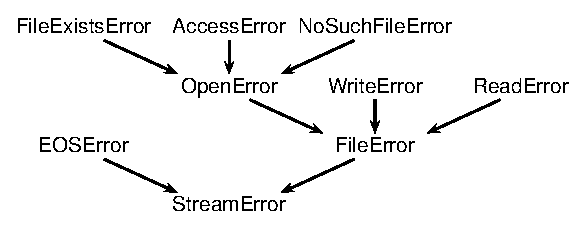
\psfig{file=extree.ps}}
\caption{Example of an exception tree structure.}
\label{exc-tree}
\end{figure}
The solution is to use two different patterns.  \cq{raise} is
used to raise an exception.  In its DO part, the \cq{deliverTo}
method can be used several times to deliver the error condition
to various exception handlers.  An exception handler is now a
direct subpattern of the \cq{exception} pattern, which is
specified as usual by a virtual binding declaration.

For the user of a library, this concept is fully backwards
compatible.  However, the writer of a library has to change the
code for raising an exception.  The exception pattern is written
such, that the old-style exception handling is still possible,
too.


\end{document}
